For a boundary component $\beta$ for $S_{g,n}$, it may be a boundary  component of different embedding pairs of pants for $S_{g,n}$. In such cases, the other two simple closed  geodesics  $\gamma_1,\gamma_2$ of the boundary components  are said to bound a pair of pants with $\beta$. For the case of $S_{1,1}$, $\gamma_1,\gamma_2$ can be the same simple closed geodesic.

Let $\{\beta_1,\cdots,\beta_n\}$ be all boundary geodesics  for $S_{g,n}$.
Define $F_{i}$ to be the set of unordered pairs  of  non-peripheral simple closed curve  isotopy classes $(\gamma_1,\gamma_2)$ which bound a pair of pants with $\beta_i$. Here the condition  $\gamma_i$ is non-peripheral requires that $\gamma_i$ is not some boundary  geodesics for $S_{g,n}$. Replace the simple closed geodesic by its isotopy class because the image of a simple  closed geodesic under a self- diffeomorphism  may not be a simple  closed geodesic,  but the isotopy class of it contains a unique simple closed geodesic. Similarly, define $F_{i,j}$ to be the set of non-peripheral simple closed geodesic  isotopy classes which bounds a pair pf pants along with $\beta_i$ and $\beta_j$.


\begin{figure}[h]
    \centering
    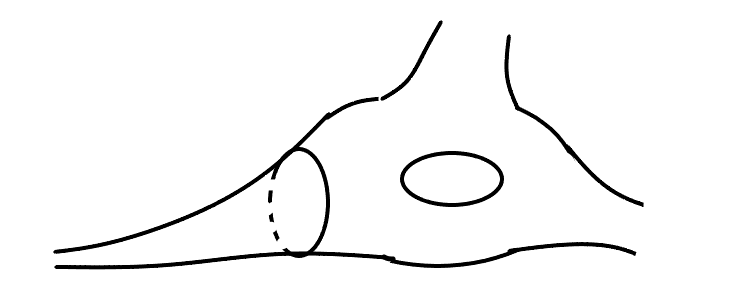
\includegraphics[width=3 in]{picture/cusp.png}
    \caption{Cusp}
    \label{fig:cusp}
\end{figure}


When the length  of some  boundary component  of the surface $S$  is zero, $S$ is a punctured  surface, and the neighborhood of the boundary component  is called a cusp. More concretely, a cusp is   the quotient domain $\{x+iy\in H|y\geq 1\}/(Tz=z+p)$ of area $p$. The horocycles $y=a$ are  corresponding to curves of length $\frac{1}{a}$ for all $a\geq 1$, they lie in the same isotopy class which contains no closed geodesic, and the minimum sequence tend to the infinity. 

For punctured surface, use $\beta_i$ to denote  the corresponding cusp instead of the boundary component, and define $F_i$, $F_{i,j}$ similarly. 




 Greg McShane prove the McShane identity in \cite{McShane1998SimpleGA} for Riemann surfaces with cusps.

\begin{theorem}[McShane identity]\label{Mcshaneid}
\begin{equation}\label{Mcshaneidorig}
    \sum_{\alpha,\beta}\frac{1}{1+\exp\left(\frac{l_\alpha(X)+l_\beta(X)}{2}\right)}=\frac{1}{2},
\end{equation}
Where the sum is taken over all the unordered  pairs $(\alpha,\beta)$ of simple closed geodesics or cusps bounding  a pair of pants with a fixed cusp. 
\end{theorem}

Mirzakhani generalizes the identity to Riemann surface with positive boundary lengths in \cite{Mirzakhani:2006fta}. 

\begin{theorem}[McShane--Mirzakhani identity]
For $X\in \mathscr{T}_{g,n}(L)$ with negative Euler characteristic,  then \begin{equation}\label{McMiid}
\sum_{\{\gamma_1,\gamma_2\}\in F_1}D(L_1,l_{\gamma_1} (X),l_{\gamma_2}(X))+\sum_{i=2}^n\sum_{\gamma\in  F_{1,i}}R(L_1,L_i,l_{\gamma}(X))=L_1.
\end{equation}
Here $L=(L_1,\cdots,L_n)$ are the length of boundary components.
\end{theorem}

Take the derivative of  the McShane--Mirzakhani identity with respect to $L_1$ at $L_1=0$ from the direction $L_1>0$. According to (\ref{pp1}) and (\ref{pp2}), the following corollary holds:

\begin{corollary}
For $X\in \mathscr{T}_{g,n}(0,L_2,\cdots,L_n)$ and $3g-3+n>0$,
\begin{equation}\label{derivMc}
    \sum_{\{\gamma_1,\gamma_2\}\in F_1}\frac{1}{1+e^{\frac{l_{\gamma_1}(X)+l_{\gamma_2}(X)}{2}}}+\sum_{j=2}^n\sum_{\gamma\in F_{1,j}}\frac{1}{2}\left(\frac{1}{1+e^{\frac{l_\gamma(X)+L_j}{2}}}+\frac{1}{1+e^{\frac{l_\gamma(X)-L_j}{2}}}\right)=\frac{1}{2}.
\end{equation}
\end{corollary}

\begin{remark}
The summation of infinity numbers and the derivation can exchange since the all terms are positive with positive derivations.
In (\ref{derivMc}), let $L_i=0$ for $i=2,3,\cdots,n$, it is the same as (\ref{McMiid}). 
\end{remark}

Note that in (\ref{McMiid}), $L_1$ is the length of boundary component $\beta_1$,  $D$ and $R$ are the length of arc on $\beta_1$ with respect to the pair of pants bounded by $\beta_1,\gamma_1,\gamma_2$ or $\beta_1,\beta_j,\gamma$. So to prove (\ref{McMiid}), separate $\beta_1$ into different pieces and calculate the length of all pieces will help. Meanwhile, it is necessity to show they are disjoint and the complement of their union is of measure zero.

A geodesic is called complete if it is not contained in another geodesic strictly. For a point $x\in \beta_i$, use $\gamma_x$ to denote the unique complete simple  geodesic passing $x$ and meeting with $\beta_i$ perpendicularly. $\gamma_x$ may the the shortest simple geodesic connecting $\beta_i$ and some $\beta_j$ in the homotopy class of finite length, it may also intersect itself at finite length and stop, otherwise it may be of infinite length and spiral around an asymptotic  geodesic.  

\begin{remark}
For a cusp domain of area $p<2$, a complete geodesic that enter it must be of the form $\{x=x_0\}$, which can be seen as orthogonal to the cusp. The original proof for McShane identity and the proof for the generalized identity are similar. 
\end{remark}


Define $E(X)$ to be the union of all simple complete geodesics which have a right intersection angle  at each meeting point with boundary components. $E_i=E(X)\cap \beta_i$ is its intersection with $\beta_i$. In figure \ref{fig:pantshy}, $y_1,y_2,z_1,z_2,w_1,w_2\in E_i$. They cut $\beta_1$ into arcs of length $\frac{1}{2}D(l_{\beta_1}(X),l_{\beta_2}(X)$, $l_{\beta_3}(X)),l_{\beta_1}(x)-R(l_{\beta_1}(X),l_{\beta_2}(X)$, $l_{\beta_3}(X)),l_{\beta_1}(x)-R(l_{\beta_1}(X),l_{\beta_3}(X),l_{\beta_2}(X))$. 
\begin{lemma}\label{measurezero}
$E_i\subset \beta_i$ is of measure zero.
\end{lemma}

\begin{proof}
Double $X$ along $\partial X$ to get $\hat{X}$. Consider the collar neighborhood $T(\beta_o)$ along $\beta_i$. Then the metric is $d\rho^2+l(\beta_i)^2\cosh^2\rho dt^2$ under the cylinder representation. For $x\in E_i$, the geodesic $\tilde{\gamma}_x$ on $\hat{X}$ passing $x$ perpendicularly is of the form $t=c$ for $c$ a constant.  For $x\neq y\in E_i$,  $\tilde{\gamma}_x\cap T(\beta_i)$ and $\tilde{\gamma}_y\cap T(\beta_i)$ are disjoint.
It follows $$\mu(\{\tilde{\gamma}_x|x\in E_i\}\cap T(\beta_i))=2 \mu(E_i)\cdot \sinh w(\beta_i)$$, where $w(\beta_i)$ is the half width of the collar $T(\beta_i)$.
By the definition of $E_i$, $\tilde{\gamma}_x$ is a  complete geodesic. By \cite{BIRMAN1985217}, the union of simple complete geodesic on $\hat{X}$ is of measure zero.
So $\mu(\{\tilde{\gamma}_x|x\in E_i\}\cap T(\beta_i))=0,$ which  implies $\mu(E_i)=0.$
\end{proof}



For $X\subset Y$, call $x\in X$ isolated if there is an open neighborhood $U$ in $Y$ of $x$ such that $U\cap X=\{x\}$. Call $x\in X$ a boundary point if $x$ is a limit point in $X$, or there exists a sequence $\{x_n\}$ of different elements in $X$ converging to $x$, and there exists a connected open set $U$ contained in $Y\backslash X$ such that $x\in \overline{U}$. Notice that this definition of boundary point is stronger than that in basic topology.


 \begin{figure}[h]
     \centering
     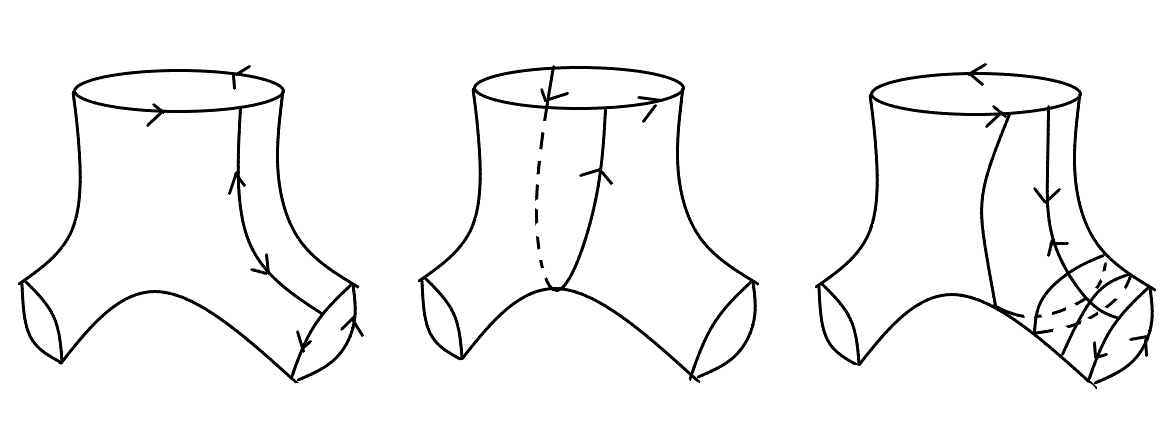
\includegraphics[width=5 in ]{picture/findpants.png}
     \caption{Pants containing $\gamma_x$}
     \label{fig:findpants}
 \end{figure}

For $x\in E_i$ connecting $\beta_i$ and $\beta_j$, there is always a canonical  method to find a pair of pants containing $\beta_i$, $\beta_j$ and $\gamma_x$.  If $\beta_i\neq \beta_j$, then consider $\beta_i\cup\gamma_x\cup\beta_j$ as a closed curve, with $\gamma_x$ twice. Among its homotopy class there is a unique simple closed geodesic $\gamma$ which bounds a pair of pants along with $\beta_i,\beta_j$. See figure \ref{fig:findpants}.  If $\beta_i=\beta_j$, then $\beta_i$ is cut into two pieces $\gamma_a,\gamma_b$, and consider the unique simple closed geodesic $\gamma_1$ in the homotopy class of $\gamma_a\cap \gamma_X$ and the unique simple closed geodesic $\gamma_2$ in the homotopy class of $\gamma_b\cap  \gamma_x$. Then $\gamma_1,\gamma_2$ bound a pair of pants along with $\beta_i$. If $\gamma_x$ spiral around $\gamma$, then is can be seen as the union of  a minimal   geodesic arc $\gamma_{x_0}$ between $\beta_i$ and $\gamma$, with an infinite  copies  of $\gamma$, find the pair of pants $P$ containing $\gamma,\beta_i$, and $\gamma_{x_0}$, then it will contain $\gamma_x$.  


According to McShane \cite{McShane1998SimpleGA}, there is a closed relationship   of topology of $x$ in   $ E_i\subset \beta_i$ and the behavior of $\gamma_x$.

\begin{theorem}\label{classify}
Points $x\in E_i$ can be classified as follows:
\begin{enumerate}
    \item If the other end of $\gamma_x$ approaches some $\beta_j$, then $x$ is isolated.
    \item If $\gamma_x$ spirals around a non-peripheral simple closed geodesic, then $x$ is a boundary point.
    \item Otherwise, $x$ is neither isolated nor a boundary point.
\end{enumerate}
\end{theorem} 

\begin{remark}


For the first case, the other end of $\gamma_x$ approach a boundary component have two possible situations. $\gamma_x$ may be the shortest geodesic connecting two boundary components and meeting them orthogonally,  or it will spiral around another boundary component and have finite length. Consider this in the pair of pants contains the geodesic and the two end boundary components.  In figure \ref{fig:pantshy}, if $\beta_1$ and $\beta_3$ are boundary components, then $y_1,y_2\in E_1$ are isolated, and the end point $x\in \beta_1$ of shortest geodesic connecting $\beta_1,\beta_3$ is isolated. For $x$, the arc $(y_1,y_2)$ which doesn't contain $w_i$, is the maximal open neighborhood the intersection of which with  $E_1$ is $\{x\}$. For $y_1$, the arc $(x,w_1)$ is the maximal open neighborhood the intersection of which with  $E_1$ is $\{y_1\}$. No matter whether $\beta_3$ is a boundary component, $w_1,w_2$ are isolated, and $(y_1,z_1)$ is the maximal open neighborhood the intersection of which with  $E_1$ is $\{w_1\}$.

For the second case, also consider it in the pair of pants contains the geodesic and the boundary component along with the asymptotic geodesic. In figure \ref{fig:pantshy}, if $\beta_3$ is non-peripheral, then $y_2,y_3\in E_1$ are boundary points, and the interval $(y_1,w_1)$ which doesn't contain $y_2$  is contained in $\beta_1\backslash E_1$. The sequence ${\gamma_{x_n}}$ contained in $E_i$, which convergent to $\gamma_{y_1}$, is   given by straightening $T^n(\gamma_x)$. Here $T\subset \Mod_{g,n}$ is the Dehn twist along $\beta_3$.  
\end{remark}




\begin{theorem}\label{Cantorset}
$E_i$ is the  union of a Cantor set and countably many isolated points.
\end{theorem}
\begin{proof}
For a subset of $[0,1]$, if it's closed with no isolated point, compact, and  totally disconnected , then 
 it is  homeomorphic to the Cantor set \cite{topologycantor} .
 
 
For isolated points in $E_i$, it is embedded into a pair of pants contained at least two boundary components, and the third boundary geodesic corresponding to  an element in the fundamental group. Since $S_{g,n}$ is a finite CW complex, by van Kampen's theorem, its fundamental group is finitely generated, so is countable.   

Notice that the Cantor set $C$ can be seen as the real number in $[0,1]$, one ternary representation $(a_0.a_1a_2\cdots)_2$ of which satisfies $a_i\neq 1$.  If $x=(a_0.a_1a_2\cdots)_2$  satisfies  only finite $a_i$ are $0$, or only finite $a_i$ are $2$, then $x\in C$ is boundary point, otherwise $x$ is not boundary point.  This corresponds to the second and third cases in theorem \ref{classify}.
\end{proof}



\begin{proof}[Proof of Theorem \ref{Mcshaneid}]
The complement of a Cantor set in $[0,1]$ is the  union of 
disjoint open intervals.

Define $I_i$  to the set of isolated points in $E_i$. By theorem \ref{Cantorset}, assume that $$
I_i\cup (\beta_i\backslash E_i)=\cup_{h}(a_h,b_h),
$$
 the union of disjoint intervals.  
 
 By definition, $a_h$ and $b_h$ are boundary points in $E_i$.
Assume that $\gamma_{a_h}$ spirals around $\Omega(\gamma_{a_h})$, which is not a boundary component.  Consider  the unique embedded pair of pants $\Sigma$ which contains $\beta_i$ and $\gamma_{a_h}$ entirely, and $$
\partial \Sigma=\{\beta_i,\Omega(\gamma_{a_h}),\gamma\}.
$$
In $S_{g,n}$, $\Omega(\gamma_{a_h})$ and $\gamma$ may overlap, but in $\Sigma$ they are cut apart and distinct. $\gamma$ may be another boundary component. 

Consider $\gamma_{b_h}$, it must spiral around $\Omega(\gamma_{a_h})$ or $\gamma$. Calculate  the length  $|b_h-a_h|$ of each interval for the two cases.

If $\Omega(\gamma_{b_h})=\Omega(\gamma_{a_h})$, then $\gamma$ must  a boundary component $\beta_j$, so $\Omega(\gamma_{a_h})\in F_{i,j}$. The interval of $(a_h,b_h)$  is of length $$ |b_h-a_h|=R(L_i,L_j,l_{\Omega(\gamma_{a_h})}(X)).$$
While if $\gamma_0\in F_{i,j}$, see $\Sigma$ in Figure \ref{fig:pantshy}. Assume  that $\beta_1$ and $\beta_2$ are boundary components of $S_{g,n}$ and $\beta_3$ is not. $\beta_3\in F_{1,2}$. Then $y_1$ and $y_2$ are boundary points in $E_1$, and they are  the limit points of a sequence in $E_1\cap (y_1y_2)$. Here $(y_1y_2)$ doesn't contain $w_i,z_i$. $E_1-[y_1,y_2]$ contains only five isolated points, $z_1,z_2,w_1,w_2$, and the meeting point of $\beta_1$ and the shortest geodesic connecting $\beta_1$ and $\beta_2$. 
 
Thus there is a one to one correspondence between intervals $(a_h,b_h)$ with $\Omega(\gamma_{a_h})=\Omega(\gamma_{b_h})=\gamma$ and $\gamma\in F_{i,j}$.


If $\Omega(\gamma_{b_h})=\gamma$, then $\gamma$ is not a boundary component and $\{\Omega(\gamma_{a_h}),\gamma\}\in F_i$. The interval $(a_h,b_h)$ is of length $$|b_h-a_h|=\frac{1}{2}D(L_i,l_{\Omega(\gamma_{a_h})}(X),l_{\gamma}(X)).$$ 
Notice that the image of $(a_h,b_h)$ under the reflection  $\sigma$ is also an open interval in $I_i\cup (\beta_i\backslash E_i)$ with the same length. So when calculate the sum of the length of all intervals, $\frac{1}{2}D(L_i,l_{\gamma_1}(X),l_{\gamma_2}(X))$ should be added twice  for $\{\gamma_1,\gamma_2\}\in F_i$.

Thus there is a two to one correspondence between intervals $(a_h,b_h)$ with $\gamma_1=\Omega(\gamma_{a_h})\neq \Omega(\gamma_{b_h})=\gamma_2$ and $\{\gamma_1,\gamma_2\}\in F_i$.
 
Since $E_i$ is of measure zero by lemma \ref{measurezero}, the $L_i=\sum_{h}|a_h-b_h|$. By the correspondence above, it is of the form 
\begin{equation*}
\sum_{\{\gamma_1,\gamma_2\}\in F_i}D(L_i,l_{\gamma_1} (X),l_{\gamma_2}(X))+\sum_{j\neq i}\sum_{\gamma\in  F_{i,j}}R(L_i,L_j,l_{\gamma}(X))=L_i.
\end{equation*}
\end{proof}
